%This file will discuss solutions implemented
%This file should be included in doc using \input{file}

\section{Proposed Solutions}
\label{proposed:simulations}
\subsection{Simulations}
For the control design, four separate controllers will be used.  A PID controller will be used to control the altitude of the quad-rotor drone.  Pitch, roll, and yaw will each be controlled respectively by a separate PI controller. These controllers will be first tested and tuned using test inputs.  The physical aspect of the simulation will be defined by a SimScape MultiBody model.  Once this rudimentary model is verified, the simulation will be developed into taking real-time signals from a HID and rendering the flight of the quad-rotor drone in response to user input.

\subsubsection{Simulation Design}
The overall architecture of the proposed design can be seen in Figure \ref{fig:sim_arch}.  The entire system is broken down into six subsystems.  Their specifications are discussed below.  The layout of each subsystem and the overall SimuLink simulation layout may be found in Appendix \ref{appendix:simulation}.

\begin{figure}[H]
	\centering
	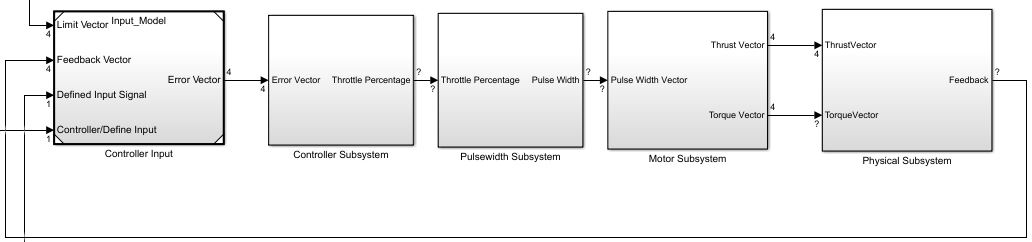
\includegraphics[width=0.9\textwidth]{system_arch.jpg}
	\label{fig:sim_arch}
	\caption{Proposed Simulation Architecture}
\end{figure}

\begin{enumerate}
	\item \textbf{Input Block:}  This block handles the HID input and pre-configured test signals.  As well as the specifications of limit/scalar values of the input signals.  As the limits will be scalar values, control signal input should be restricted between $-1$ and $1$.
	
	\item \textbf{Feedback Block:}  This block receives the contents specified from the input block as well as the current orientation of the quad-rotor drone in the simulation.  It combines all of these to output an error signal for the pitch, roll, yaw, and altitude controllers.
	
	\item \textbf{Controller Block:}  This block houses the four controllers.  The output of these controllers is normalized to a throttle percentage.
	
	\item \textbf{Pulsewidth Subsystem:}  This block takes the throttle percentage and transform it to a value in microseconds that can be used to define the pulsewidth output of the microcontroller.  Physically, this PWM signal controls the ESCs.
	
	\item \textbf{Motor Characterization:}  This block contains motor thrust data corresponding to characterization tests performed in the first semester.  Functionally this block contains a look up table that relates pulsewidth to thrust and torque for each motor.  The torque value is an approximation based on the value of thrust from the motor.
	
	\item \textbf{Physical Subsystem:}  This block contains the physical subsystem built in SimScape Multibody.  This library allows for the system to be built quickly and easily, as well as providing a (although simple) 3D rendering model.
	
	\item \textbf{3D Rendering:}  This subsystem will handle the real-time rendering of the simulation for flying with input from the HID.
\end{enumerate}

\subsection{Physical Implementation}

The proposed solution incorporates the following components for the physical system architecture.

\begin{itemize}
\item Joystick Controller
\item Base Station Laptop
\item Raspberry Pi 3 Computer
\item Arduino Micro-Controller
\item 10 Degree of Freedom Inertial Measurement Unit
\item Raspberry Pi Camera Module (Future)
\end{itemize}

The system architecture is implemented as depicted in the block diagram shown in Figure \ref{fig:sys_arch}. 

\begin{figure}[H]
	\centering
	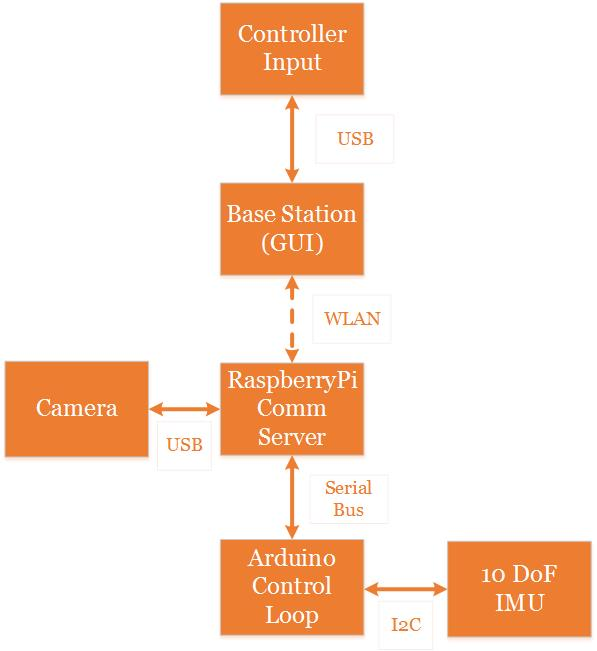
\includegraphics[width=0.7\textwidth]{flowchart-architecture.jpg}
	\caption{System Architecture}
	\label{fig:sys_arch}	
\end{figure}

A joystick controller was used as the control input for its non-spring loaded throttle control. The drone requires an altitude set point from the control input, a spring loaded control input would make the implementation of a constant set point difficult. The base station laptop hosts the GUI and the communication channel software between the USB connected joystick control input and the Raspberry Pi Wi-Fi connection. The Python scripts that enable the communication channels use the sockets library for a server, client Wi-Fi channel and pygame library to acquire control set points from the joystick controller. The inputs from the controller are converted from floats to sets of four bytes for transmission.

The Raspberry Pi is used solely as a communication channel between the base station and the Arduino control loop. The RPi is the server while the base station is considered the client in the connection. The Raspberry Pi relays the received bytes to the Arduino control loop using a serial communication channel. 

The Arduino control loop is used to host the drone function library and main script required for drone flight. The Arduino control loop outline is shown in Figure \ref{fig:ctl_loop}. The gain values for the PID loop are to be determined through simulations. The Arduino initializes all sensors, motors, and communications. The loop then gathers data from the inertial measurement unit and the serial connection to the Raspberry Pi, compares the data and performs PID loops, finally outputting the results to the ESCs.

\begin{figure}[H]
	\centering
	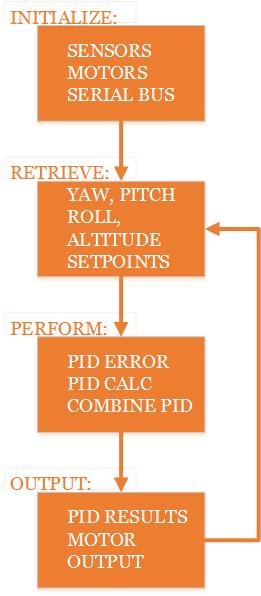
\includegraphics[width=0.3\textwidth]{control-loop.jpg}
	\caption{Arduino Control Loop}
	\label{fig:ctl_loop}	
\end{figure}

Yaw, pitch, roll and altitude are calculated using the accelerometer, gyroscope, magnetometer, barometric pressure sensor and temperature sensor available on the inertial measurement unit. The altitude measurement is completed using the barometric pressure sensor and temperature sensor. The equation to calculate altitude is given as: 

\vspace*{0.2in}
$h=\frac{(\frac{P_{0}}{P})^\frac{1}{5.257}-1)*(T+273.15)}{0.0065}$
\vspace*{0.2in}

$h$ = Difference between Starting Height and Current Height

$P_{0}$ = Initial Pressure at Starting Height

$P$= Current Pressure

$T$ = Current Temperature

\vspace*{0.2in}

The barometric pressure sensor calculation was found to be highly susceptible to noise, several filtering techniques were attempted and a Kalman filter with a feedback comparison is currently in use. This filtering technique is subject to change. All written scripts for the Arduino, Raspberry Pi and the base station communication channel can be found in Appendix B. 

The hardware build of the drone requires mounting the Arduino and Raspberry Pi on the drone, connecting the 10 DOF IMU to the Arduino through an I2C connection, ESC connections through the available PWM pins on the Arduino, and a serial connection to the Raspberry Pi. The ESCs are to be powered by a lithium ion battery through a power distribution board. The power distribution board will also provide power supply to the Raspberry Pi, supplying power to the Arduino through the serial USB connection.

The PID loop implementation utilizes the Forward Euler equation. The scripted solution to the PID loop can be seen in Appendix B and the mathematical breakdown is as follows. Note, the forward Euler equation is manipulated algebraically to obtain the numerator and denominator coefficients. 

\begin{align*}
          Forward Euler &= k_P+k_I * T_s * \frac{1}{z-1} + k_D * \frac{N}{1+N*T_s*\frac{1}{z-1}} \\
           C(z) & = \frac{U(z)}{E(z)} = \frac{b_0 +b_1z^{-1}+b_2z^{-2}}{a_0 +a_1z^{-1}+a_2z^{-2}}\\
           \\
          b_0 & = k_P(1-N*T_s) + k_I*T_s(N*T_s-1)+k_D*N \\
          b_1 & = k_P(N*T_s-2) + k_I*T_s+2*k_D*N \\
          b_2 & = k_P+k_D*N \\
          a_0 & = 1-N*T_s \\
          a_1 & = N*T_s-2 \\
          a_2 & = 1 \\
\end{align*}

The implemented difference equation is denoted u[k].

\begin{align*}
u[k] & = -\frac{a_1}{a_0} u[k-1] - \frac{a_2}{a_0} u[k-2] + \frac{b_0}{a_0} e[k] +\frac{b_1}{a_0} e[k-1] +\frac{b_2}{a_0} e[k-2]  
\end{align*}


\subsection{Graphical User Interface}
\subsubsection{Framework Selection}
The basic GUI was to have the ability to call the joystick initialization script and manipulate the axis settings. Because the initialization script was written in Python it was very difficult and time consuming to do this using the C++ version of Qt compared to using PyQt5 where all that had to be done was import the script. Due to each of the scripts that the GUI needs to call are written using Python it was decided to carry on using PyQt5. On top of the ease of importing the scripts using PyQt5 it also allows us to use the vast amount of Python libraries that are available such as matplotlib and pyqtgraph and as discussed, these libraries will be used to plot the sensor data. 
\subsubsection{Features}
As mentioned in section 3.3.2 how we could go about implementing each of the listed features was researched. Through this research is was revealed that some of the features we had originally considered were out of the scope of this project because it would take too much time to implement for little benefit. For this reason the following features were removed from our consideration at this time, but they will be considered potentional future improvements: 
\begin{itemize}
	\item Manipulate and Display PI and PID Parameters
	\item Display Sensor Status
	\item Display Flight Time
\end{itemize}
Therefore the key features that will be implemented into the GUI at this time are as follows:
\begin{itemize}
	\item Initialize Manual Control of the Drone
	\item Initialize communications between Base Station Host and Raspberry Pi 3
	\item Display Live Plots
\end{itemize}
A detail explanation of how these features will be implemented into the GUI will be explained in sections 4.3.4-4.3.5.
\subsubsection{GUI Layout}
As explained in section 3.3.3 an initial GUI was developed and presented to our client this initial prototype can be viewed in Appendix \ref{appendix:gui} Figure \ref{fig:oldgui1} and Figure \ref{fig:oldgui2}. As you can see from the figures in \ref{appendix:gui} the prototype presented to our client included most of the features we later deemed unnecessary therefore we could disregard these extra widgets. With the decision to not include the features and taking our clients comments into consideration a new GUI layout was developed. The new GUI layout includes all of the key features we have decided to implement and presents them in a clean and intuitive manner. This new layout was presented to each group member and a consensus was reached to carry on with development using this layout. The final GUI layout can be viewed in Figure \ref{fig:GUIHome} and Figure \ref{fig:GUICtrl}.
\begin{figure}[H]
	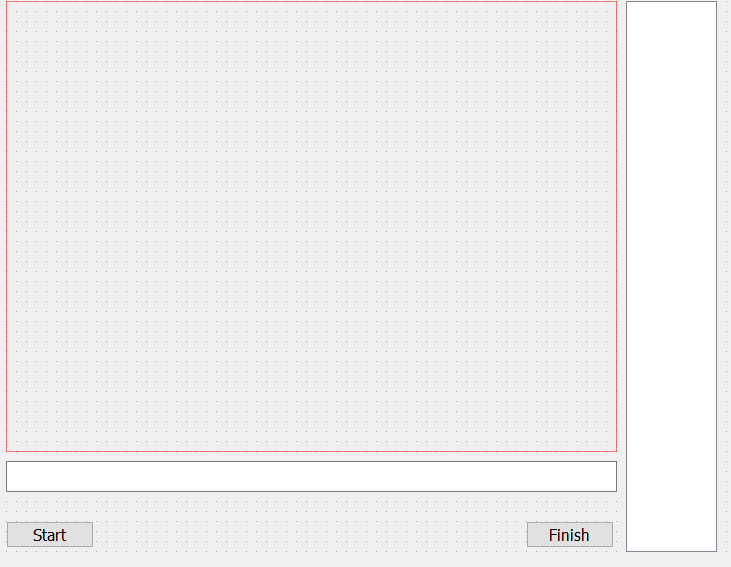
\includegraphics[width=\linewidth]{Final_GUI_HOME.png}
	\caption{Final GUI Home Page}
	\label{fig:GUIHome}
\end{figure}
\begin{figure}[H]
	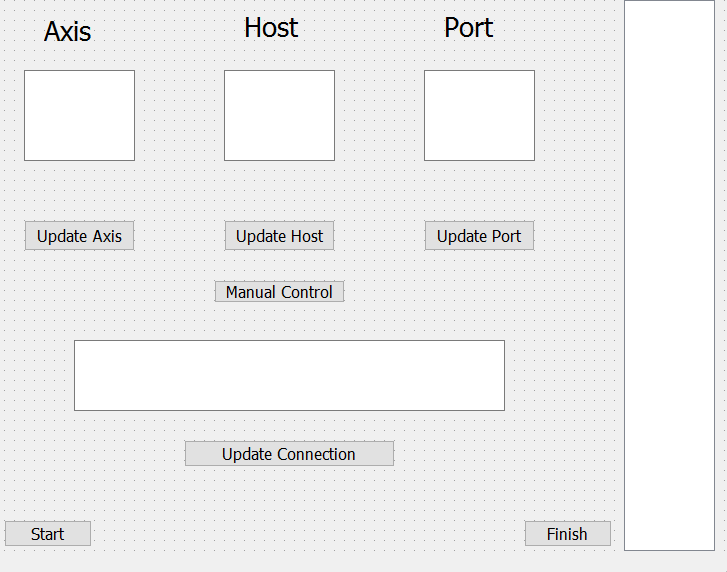
\includegraphics[width=\linewidth]{Final_GUI_CTRL.png}
	\caption{Final GUI Controller and Network Settings page}
	\label{fig:GUICtrl}
\end{figure}
The red outlined box is the field that the live plot will populate when the GUI is compiled and the blank vertical rectangle is a list widget that will be populated with the names different pages of the GUI and will allow the user to access them by simply clicking on the name. An example of how the list widget will look can be viewed in Figure \ref{fig:list} and how the live plot will look can be viewed in section 4.3.5 Figure \ref{fig:plt}. An explanation of what purpose each of the other widgets and push buttons seen in Figures \ref{fig:GUIHome} and \ref{fig:GUICtrl} will serve is described in the following sections.
\begin{figure}[H]
	\centering
	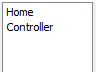
\includegraphics[width=0.3\linewidth]{listWidget.png}
	\caption{List Widget Example}
	\label{fig:list}
\end{figure}
\subsubsection{Initializing Communications and Manual Control}
In order for the GUI to receive sensor data or the controller to receive manual control inputs over WiFi a socket connection must be made. Instead of having to open and run the socket script on the client (base station host in our case) the Start button on the GUI calls the socket script and makes the connection to the socket. Once the Start button has been pressed the horizontal white fields found in Figures \ref{fig:GUIHome} and \ref{fig:GUICtrl} will tell the users whether or not communications have been successfully made how this push is coded can be found in the connection() definition of the GUI code in Appendix C.1. When the GUI is initially compiled the white fields under Axis and Port seen in Figure \ref{fig:GUICtrl} will be populated with the default values that are found in the Joystick script found in Appendix B.3 Listing 5 for the Axis values and the socket script for the Port value. The white field under Host will be populated with the name of the host computer's IP or name. 

The Axis values will determine which direction the drone will go depending on which way to joystick is moved therefore if the user would prefer the drone move differently they have the option to change the joystick settings by hitting the "Update Axis" push button. How this push button is coded to achieve this functionality can be found in the updateAxis() method in the GUI code in Appendix C.1

In the event that the client script is altered and a new host and port number is to be used for the socket the "Update Connection" push button will allow the user to enter the new host and port values and then the connection to the new socket will be made. If only one value has changed the user can select either the "Update Host" or "Update Port" push buttons and then hit "Update Connection" and the new connection will be made. If either of these cases occur the horizontal white field found in Figure \ref{fig:GUICtrl} will be populated letting the user know whether or not the values have been updated and the connection has been successfully established. How the Axis value, Host value, Port value and Connection Status will be displayed when the GUI is compiled and the Start button is pushed using the wrong port value can be viewed in Figure \ref{fig:guipop1} and how the text field that pops up when you click any of the push buttons mentioned looks can be viewed in Figure \ref{fig:popup}

\begin{figure}[H]
	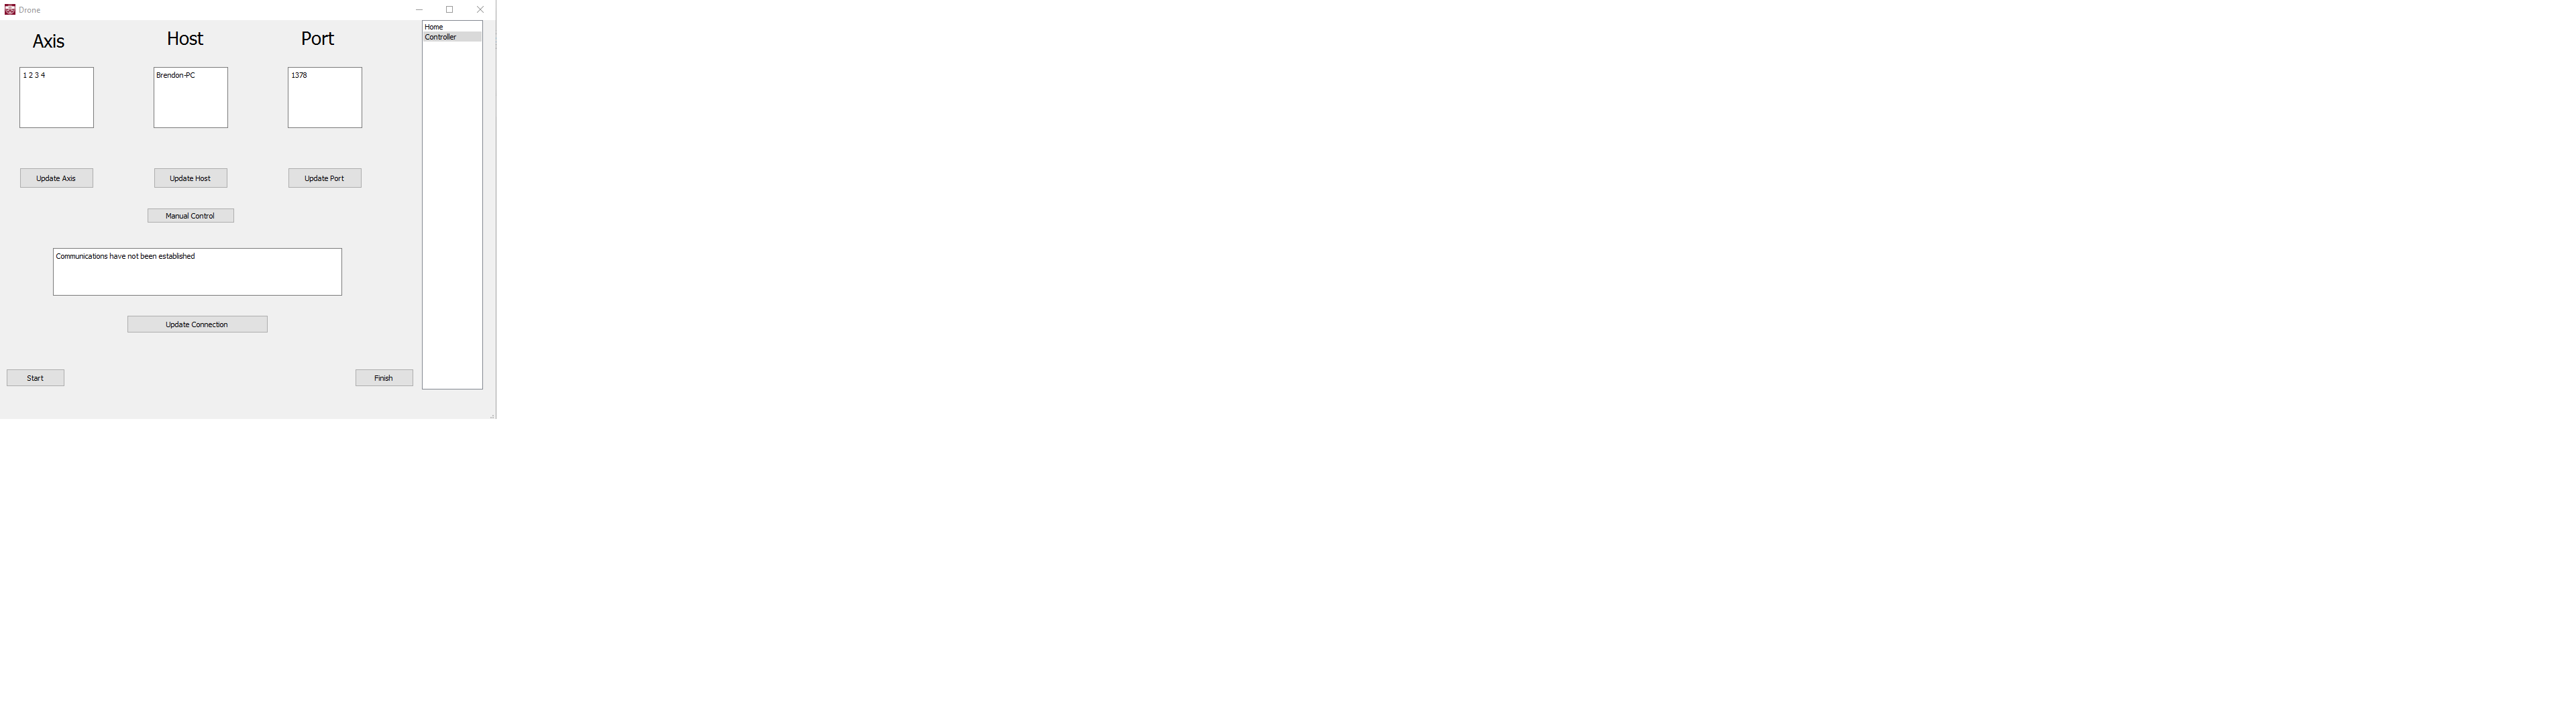
\includegraphics[width=\linewidth]{GUICtrlPop.png}
	\caption{Compiled GUI with no active communications}
	\label{fig:guipop1}
\end{figure}

\begin{figure}[H]
	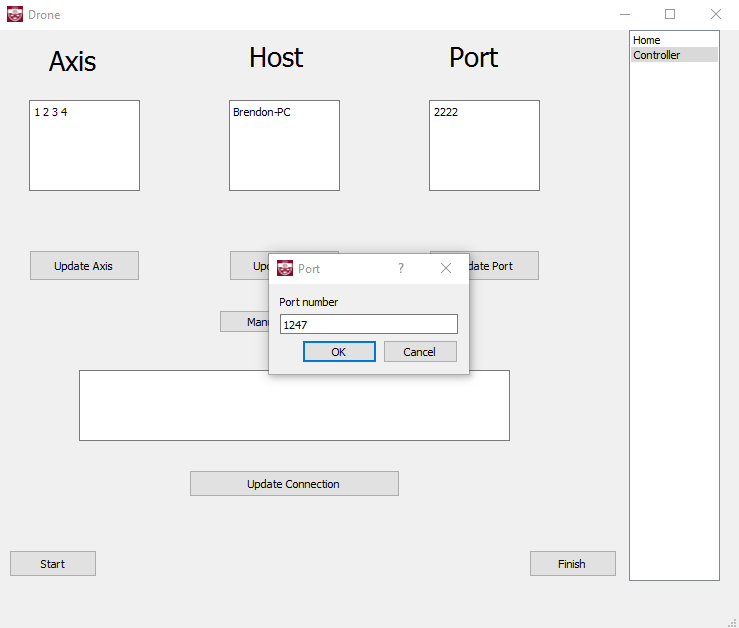
\includegraphics[width=\linewidth]{GUIPopup.png}
	\caption{Pop up to input new values on GUI}
	\label{fig:popup}
\end{figure}

As mentioned in section 2.1 Dr. Rhinelander has aspirations for the drone to partially or fully fly on it's own but in the event that something goes wrong there must be a way to manually control the drone. This is where the manual control button seen in Figure \ref{fig:GUICtrl} comes into play. This push button calls the listen() definition of the Joystick initialization script found in Appendix B.3 Listing 5. This initializes the joystick settings and then makes the connection to the socket on the Raspberry Pi 3 this will allow for control inputs to be sent. In order for this to be performed the Server script found in Appendix B.2  must be running on the Raspberry Pi 3 and the port numbers must match. The code for how this push button performs it's functions can be found in the connectController() definition on the GUI code found in .

\subsubsection{Live Plotting}
As discussed in section 3.3.4 the libraries matplotlib and pyqtgraph were considered when trying to determine how to display the live plots on the GUI. When it came to just displayed a simple graph matplotlib integrated seemlessly into the GUI and looked clean. However, when it came time to update the plot a big problem was encountered this was whenever an update timer was connected to the plotting definition the instance of the plot window would repeat itself rather than pulling the data and updating the plot with the new values. Upon researching solutions to this issue it was discovered that when dealing with real time plots matplotlib has a real weakness but that pyqtgraph excels in this aspect. With these reasons combined it was decided that moving forward all live plotting will be performed using pyqtgraph.

When using pyqtgraph live plotting became much easier to achieve. To achieve live plotting three definitions are required to set up the initial plot, what to do when the plot updates and which direction to move the plot. These definitions can be found in the initplt(), update1() and move() definitions in the GUI code in Appendix C.1. Once these definitions are defined a QTimer must be connected to the move() definitions and an update interval will be defined the external dependancies and QTimer setup can be found under "Live Plotting" in the GUI code in APPENDIX. How the plot will look on the GUI can be seen in Figure \ref{fig:plt}.

On top of pyqtgraph being easier to implement it also includes some useful features. The user is able to click on the plot window and drag in any direction. For example, if the user was interested in data that occurred at time = 0 seconds but they were 100 seconds into data collection they would be able to click and drag back to the desired point to see the data of interest without disrupting data collection. If the user left clicks they are also to instantly obtain the maximum and minimum X and Y values, or in our case maximum time and amplitude values an example of the can be viewed in Figure \ref{fig:plot2}
\begin{figure}[H]
	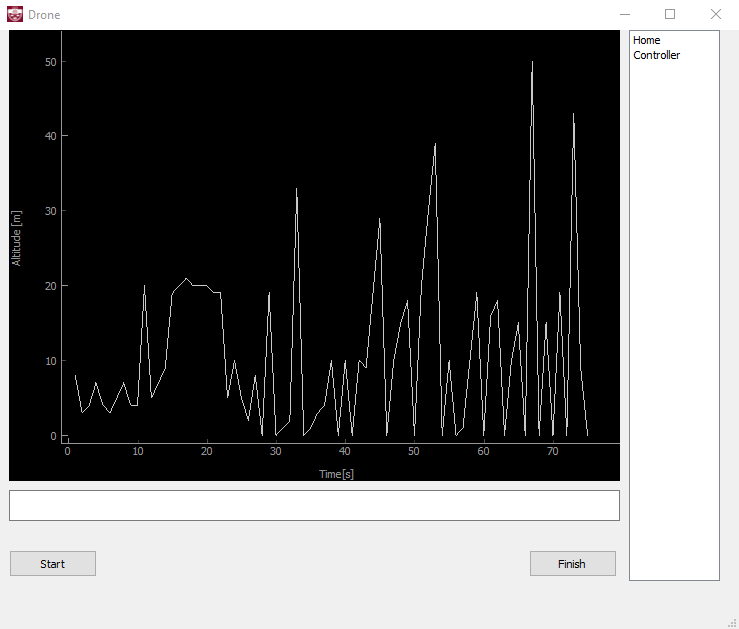
\includegraphics[width=\linewidth]{plot.png}
	\caption{Live Plot}
	\label{fig:plt}
\end{figure}
\begin{figure}[H]
	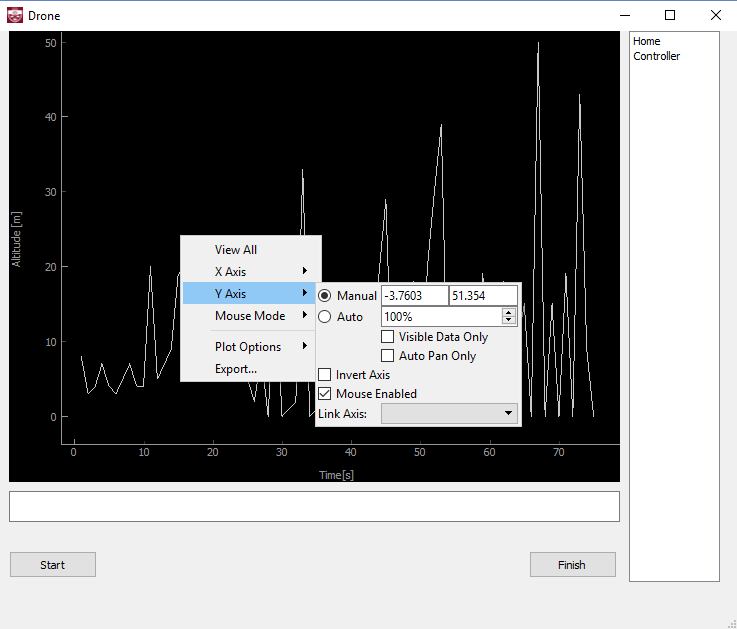
\includegraphics[width=\linewidth]{plot2.png}
	\caption{Display Y Values on Live Plot}
	\label{fig:plot2}
\end{figure}
